% ---------------------------------------------------------------
% ---------------------------------------------------------------
% This template was developed for the working paper series of 
% the Interdisciplinary Laboratory of Computational Social Science (iLCSS)
% at the University of Maryland, College Park

% The template was built based on  the PNAS Latex model. 

% Adjustments were made by Tiago Ventura, Ph.D. Student in Political Science at UMD, 
% and researcher at the iLCSS.

\documentclass[9pt,twocolumn,twoside]{ilcss}
\usepackage{listings}
\usepackage[toc,page]{appendix}


\templatetype{ilcssworkingpaper} % Choose template 

\title{M\'etodos de aprendizaje de \'maquina para inferir el nivel de cobertura de banda ancha fija en municipios  de M\'exico}	

% Use letters for affiliations, numbers to show equal authorship (if applicable) and to indicate the corresponding author
\author[a]{C\'esar Zamora Mart\'inez}
%\author[b,1,2]{Author Two} 
%\author[a]{Author Three}

\affil[a]{Alumno de Maestr\'ia en Ciencias de Datos (ITAM)}
%\affil[b]{Affiliation Two}
%\affil[c]{Affiliation Three}

% Please give the surname of the lead author for the running footer
\leadauthor{C\'esar Zamora Mart\'inez} 

% Please add here a significance statement to explain the relevance of your work
%\significancestatement{Authors must submit a 120-word maximum statement about the significance of their research paper written at a level understandable to an undergraduate educated scientist outside their field of speciality. The primary goal of the Significance Statement is to explain the relevance of the work in broad context to a broad readership. The Significance Statement appears in the paper itself and is required for all research papers.}

% Please include corresponding author, author contribution and author declaration information
%\authorcontributions{Please provide details of author contributions here.}
%\authordeclaration{Please declare any conflict of interest here.}
%\equalauthors{\textsuperscript{1}A.O.(Author One) and A.T. (Author Two) contributed equally to this work (remove if not applicable).}
\correspondingauthor{\textsuperscript{2}E-mail: czamora5\@email.itam.mx}

% Keywords are not mandatory, but authors are strongly encouraged to provide them. If provided, please include two to five keywords, separated by the pipe symbol, e.g:
%\keywords{Aprendizaje de Máquina $|$ Banda Ancha $|$ Telecomunicaciones $|$ ITAM} 

\begin{abstract}Aunque en fechas recientes se reconoce el impacto benéfico que la banda ancha tienen sobre en entorno económico y social, la penetración de tales servicios en los municipios obedece a múltiples factores que inciden en el despliegue de la infraestructura que permite su prestación. Motivado por ello, en este trabajo se plantea el uso de métodos basados en aprendizaje de máquina que permitan clasificar los municipios conforme a su nivel de  cobertura a través de indicadores de penetración y establecer factores que propician o desincentivan los despliegues de banda ancha fija.
\end{abstract}

%\dates{This manuscript was compiled on \today}

% You can change the link on the footer here

%\doi{\url{http://ilcss.umd.edu/}}

\begin{document}

\maketitle
\thispagestyle{firststyle}
\ifthenelse{\boolean{shortarticle}}{\ifthenelse{\boolean{singlecolumn}}{\abscontentformatted}{\abscontent}}{}

% If your first paragraph (i.e. with the \dropcap) contains a list environment (quote, quotation, theorem, definition, enumerate, itemize...), the line after the list may have some extra indentation. If this is the case, add \parshape=0 to the end of the list environment.

\dropcap{D}urante las últimas tres décadas las telecomunicaciones han tenido un avance sin precedentes en el mundo, posicionándose como herramientas que potencian el desarrollo económico y social, pues, como ha sido ampliamente documentado en la literatura (\cite{PRADHAN2014634}), permiten crear oportunidades, reducir la pobreza e impulsar el progreso económico y social para el bienestar de la población\footnote{\cite{Katz2018} muestra que un avance del 1\% en un índice sobre digitalización, genera un incremento de la productividad que redunda en un crecimiento económico de un 0.3\% del PIB. }. Uno de los ejes que permiten explicar lo anterior es el impacto benéfico de los servicios de banda ancha en los procesos productivos, financieros y en general el bienestar de la población (\cite{Katz2012}).

En México, a cerca de cuatro años de la reforma a de telecomunicaciones en 2013, que llevo a la promulgación de la Ley Federal de Telecomunicaciones y Radiodifusión (LFTyR) junto con la creación del Instituto Federal de Telecomunicaciones (IFT), se estimó un crecimiento superior al 37\% en las conexiones de banda ancha fija (BAF), traduciéndose a que para entonces casi la mitad los hogares contaban con servicios de Internet (\cite{IFT2017} e \cite{IFT2018}).

Aunque este fenómeno revela una tendencia favorable con respecto al entorno internacional\footnote{A finales de 2018 México fue el cuarto país con mayor crecimiento de penetración de banda ancha fija entre los países de la Organización para la Cooperación y Desarrollo Económicos (OCDE); y mostró un crecimiento de 17.9\% en la penetración de accesos por medio de fibra óptica (\cite{IFT2019})}, la Encuesta sobre Disponibilidad y Uso de Tecnologías de la Información y la Comunicación en los Hogares 2018 (ENDUTIH 2018, \cite{ENDUTIH2018}) dejó en claro la existencia de una brecha en la adopción de estos servicios para la población mexicana (por tanto en sus conducentes beneficios), pues sólo cerca de 65.8\% de la población con seis años o más es usuario de servicios de Internet en los hogares del país, además de que mostró que este es un fenómeno urbano, puesto el 73.1\% del total de la población urbana son usuarios de este servicio en contraste con la población conectada en zonas rurales que es cercana a 40.6\%.

A efecto de explicar el entorno de la penetración de servicios de Internet a nivel municipal, en adelante nos centraremos en los servicios de banda ancha fija\footnote{Ello dado que desafortunadamente, el Banco de Información de Telecomunicaciones (BIT) del IFT sólo posee el detalle desagregado de servicios de Internet de banda ancha móvil para nivel estado, sin que se hayan podido localizar fuentes con datos precisos al respecto.}, los cuales son servicios de acceso a Internet y transmisión de datos orientados a usuarios finales (personas físicas o empresas), que se brindan a través de equipos terminales (módems, terminales ópticas y demás) que tienen una ubicación geográfica determinada y fija (\cite{IFT2018man}). Ello obliga a los operadores de telecomunicaciones interesados a realizar inversiones que les permitan alcanzar los puntos geográficos en donde se localizan los clientes potenciales, esto es, cerca de hogares y edificios de empresas, aprovechando las capacidades de las tecnologías en las que se basan sus redes. 

Dicho contexto les condiciona a establecer un circuito físico o virtual a través del cual se pueda conectar la ubicación del usuario a la red del operador y a través del que se prestarán los servicios (“Acceso de datos” o simplemente como “acceso”, \cite{IFT2018man}). Por ende, dado que afrontan costos considerables en infraestructura, equipos, permisos y recursos humanos para poder brindar servicios\footnote{En línea con \cite{IFT2017reb}, no sólo se enfrentan costos directos, sino oportunidad y de transacción; así como el riesgo de afrontar costos hundidos.}, típicamente los operadores concentran su oferta en zonas densamente pobladas donde existe suficiente capacidad económica para asegurar no solo que recuperarán sus inversiones sino que serán rentables desde la visión de negocio.

Además de los aspectos socio-económicos, también se destacan otros factores que pueden ser tomados en cuentan por un operador para evaluar una zona como idónea para brindar servicios: 1) Viabilidad de permisos para desarrollar los despliegues (e.g. concesiones para operar, medio ambiente), 2) viabilidad tecnológica (e.g. limitadas técnicas por la distancia que limitan la velocidad, calidad, entre otras), 3) existencia de infraestructura cercana a la zona de la que puedan disponer para proveer servicios (por ejemplo, propia o arrendada); y 4) existencia de competencia en el área; es decir de proveedores de servicios de telecomunicaciones.
%	
%Por otro lado, un indicador ampliamente usado en el sector de telecomunicaciones (\cite{Hanafizadeh},\cite{IFT2017reb},\cite{IFT2018man}) para cuantificar la cobertura de banda ancha fija es medir la penetración en una zona con la cantidad de accesos en ella por cada 100 hogares:
%\begin{equation}\label{pen_hogares}
%PenBAFHogares = \frac{Accesos }{Hogares} \times 100 
%\end{equation}
%
%Este indicador tiene las siguientes limitaciones 1) la presencia de accesos en un municipio no implica necesariamente que las localidades que lo conforman cuentan con infraestructura para brindar estos servicios \footnote{A guisa de ejemplo, puede ser el caso que únicamente existan servicios de BAF en la cabecera municipal, pero no en el resto de sus comunidades}, 2) la penetración se puede subestimar si no se tienen un división explícita entre accesos de usuarios residenciales y empresariales.
%
%En vista de este último punto, 

Para cuantificar la cobertura de banda ancha fija la OCDE define una medida de penetración en una zona como la cantidad de accesos en ella por cada 100 habitantes, el cual es un proxy del indicador de suscriptores por cada 100 habitantes\footnote{http://www.oecd.org/internet/broadband/broadband-faqs.htm}:
\begin{equation}\label{pen_habitantes}
PenBAFHabitantes = \frac{Accesos }{Habitantes} \times 100 
\end{equation}

En este sentido, de acuerdo a la información publicada por este organismo a diciembre de 2018, sus países miembros contaban con una penetración media de 30.92 accesos por cada 100 habitantes, ocupando México el penúltimo lugar (con 14.83 accesos por cada 100 habitantes).

Por otro lado, para BAF los accesos se basan típicamente en las tecnologías\footnote{También existen configuraciones híbridas} (\cite{moya2014telecomunicaciones}): 1) DSL: tecnología de transmisión por cable trenzado de cobre, su disponibilidad y la velocidad dependen de la distancia; 2) Cable coaxial: se forma por dos hilos de cobre cuya estructura permite permite, en generala más capacidad para transmitir información que el par trenzado de cobre; 3) Fibra óptica: formados por un medio de vidrio o polímero que permite el paso de haces de luz, pueden transmitir más de 10 Gbit/s hasta a 10 kilómetros de distancia, 4) Otras: incluye uso de ondas electromagnéticas como microondas, señales satélites y demás; usualmente  tienen menor desempeño comparado a 1), 2) o 3), pero son viables en regiones de difícil acceso.

Con todo lo anterior, el objetivo del presente documento será plantear un modelo con métodos de aprendizaje de máquina que permitan identificar variables útiles para explicar el nivel de penetración de BAF (por ejemplo, datos geográficos y demográficos) así como de los factores que inciden en los despliegues de tecnologías capaces de dar servicios de Internet de alta velocidad. 

En este sentido, con motivo de estudiar a los municipios que cuentan penetración de BAF basada en tecnologías capaces de dar servicios de velocidad alta, se enfocarán los indicadores de penetración presentados previamente sobre accesos correspondientes a tecnologías de cable coaxial o fibra óptica (es decir, se calcularan con respecto la cantidad de accesos resultado de sumar de los que correspondan a cable coaxial y aquellas de fibra óptica en cada municipio).

\section{Revisión y análisis de fuentes de datos asociados a banda ancha fija}

A continuación se resumen las fuentes de información consultadas con relación a servicios de BAF, junto con las consideraciones particulares derivadas de su exploración\footnote{El procesamiento de la información se llevó a cabo a través de scripts en Bash, R y Python, véase apéndice}. 

\subsection{Revisión de fuentes de información}

En términos generales, la revisión abarcó datos públicos 
de fuentes gubernamentales y organismos internacionales relativos a siguientes los ejes:

\subsubsection{Identificación de municipios}

Dado que la disponibilidad de información social y demográfica en fuentes públicas con desglose municipal se encuentra limitada a ejercicios estadísticos que abarcan hasta el año 2015 (\cite{Intercensal2015}, \cite{CONAPO2015}, \cite{ONU2015}), la identificación de los municipios se hizo de manera congruente el marco metodológico de la Encuesta Intercensal 2015 en donde se contabilizaron un total de 2,457 municipios.

\subsubsection{Datos de accesos de banda ancha}

El Banco de Información de Telecomunicaciones (\cite{IFT2019BIT}) posee datos históricos (de 2013 a mediados 2019) sobre los accesos de banda ancha móvil y fija de México; sin embargo únicamente en el segundo caso se ofrece el detalle a nivel municipio. Dicha fuente provee datos de 29 empresas a las que pertenecen los accesos de BAF junto tecnología correspondiente (DSL, cable coaxial, fibra óptica, satelital y otras), sin proveer el desglose entre accesos residenciales o no residenciales. Se consideró relevante extraer los datos accesos en cada municipio, agregando los datos de todos los operadores por tecnología de acceso para el periodo con información más reciente (junio de 2019).

\subsubsection{Datos socio-económicos}
A través de la Encuesta Intercensal 2015 (\cite{Intercensal2015}), el INEGI reúne información de componentes que describen la evolución de la población, junto con sus viviendas y de sus condiciones socio-económicas.Tras estudiar esta fuente, los datos que se han considerado de interés para el estudio a nivel municipal la penetración de BAF son: 1) número de hogares, 2) número de habitantes, 3) porcentaje de viviendas que cuentan con disponibilidad de servicios de telecomunicaciones (es decir, a través de telefonía fija, telefonía celular, televisión de paga e Internet)\footnote{Ante la ausencia de información pública sobre la presencia de infraestructura (ver \cite{IFT2017reb}) que permita proveer servicios de Internet de alta velocidad, por ejemplo la localización de centrales de redes de nueva generación o la presencia física de la red backhaul/core de los principales operadores de México o CFE, se estima que la información indirecta de la presencia de servicios constituye un proxy para la presencia de infraestructura necesaria, aunque no suficiente, para poder brindar tales servicios a usuarios finales. A su vez, dicha elección se apoya en que, como se ha mencionado previamente, los despliegues de redes fijas se realizan alrededor de donde se ubican los clientes potenciales, y a su vez en el hecho de que la presencia de servicios de telecomunicaciones (incluso distintos a BAF) constituye una señal de que existen condiciones positivas para que los operadores desarrollen una cadena de elementos de infraestructura y operación que le permitan atender en una zona específica ofreciendo servicios a la población}. 


\subsubsection{Datos asociados a marginación}

La Comisión Nacional de Población (CONAPO) diseño una herramienta denominada "índice de marginación" para realizar mediciones de las carencias que padece la población (\cite{CONAPO2015}). Esta recoge una serie de dimensiones socio-económicas para su construcción: educación, vivienda, y distribución de la población e ingresos. Para explorar la relación de tales ejes con la penetración de servicios de BAF, se consideró relevante involucrar a las siguientes mediciones empleadas por CONAPO en 2015 para la construcción de dicho índice a) porcentaje de ocupantes en viviendas sin energía eléctrica, b) porcentaje de población en localidades con menos de 5,000 habitantes, y c) porcentaje de población ocupada con ingresos de hasta 2 salarios.

%\begin{itemize}
	%\item Porcentaje de población de 15 años o más analfabeta,	
	%\item Porcentaje de población de 15 años o más sin primaria completa,	
	%\item Porcentaje de ocupantes en viviendas sin drenaje ni excusado,	
	%\item Porcentaje de ocupantes en viviendas sin energía eléctrica,\vspace{-0.1cm}	
	%\item Porcentaje de ocupantes en viviendas sin agua entubada,	
	%\item Porcentaje de viviendas con algún nivel de hacinamiento,	
	%\item Porcentaje de ocupantes en viviendas con piso de tierra,	
	%\item Porcentaje de población en localidades con menos de 5,000 habitantes,\vspace{-0.3cm}	
	%\item Porcentaje de población ocupada con ingresos de hasta 2 salarios.\vspace{-0.2cm} mínimo.	
%\end{itemize}

La elección de tales variables se basa en que: a) la energía eléctrica es una condición necesaria para el funcionamiento de los servicios de telecomunicaciones, b) los operadores deben de hacer mayores esfuerzos para atender zonas que son bajamente pobladas donde puede no ser rentable llevar servicios, y c) el ingreso de las personas constituye una condición necesaria para que puedan solventar el pago de un servicio de Internet.
 
\subsubsection{Datos asociados a desarrollo humano}

El Programa de las Naciones Unidas para el Desarrollo (PNUD) es una organización orientada a generar soluciones a los países que buscan alcanzar sus metas de desarrollo y lograr los objetivos compartidos con la comunidad internacional. Como parte de sus actividades en México \cite{ONU2015}, periódicamente evalúan el nivel de desarrollo de los municipios a través de la construcción del "Índice de Desarrollo Humano (IDH)", el cual considera los ejes de salud, educación e ingreso. Al respecto, puesto que el ingreso de la población es un componente relevante en el acceso a servicios de telecomunicaciones, se considerarán los datos del PNUD empleados para la estimación del IDH correspondientes al año 2015 relativos el ingreso bruto per cápita en poder de paridad de compra (PPC), expresado en dólares estadounidenses, de cada municipio\footnote{Estos datos no se encuentra disponibles para 11 municipios. 
	A saber 5 del estado de Chihuahua (Buenaventura, Carichí, Santa Isabel, Temósachic, y Urique), 4 en Oaxaca (Matías Romero Avendaño, Santa María Chimalapa, Santa María Petapa y San Francisco Chindúa), uno en Puebla (San Nicolás de los Ranchos) y otro en Sonora (General Plutarco Elías Calles)
}.

\subsection{Consideraciones sobre la información reunida}

En términos de la información reunida, la exposición previa (así como la metodología propuesta por \cite{IFTcobertura2018}), el análisis de cobertura para servicios de BAF partirá de las siguientes premisas:

\begin{itemize}
	\item \textbf{Periodo de la información de accesos:} junio de 2019,\vspace{-0.2cm}
	\item \textbf{Nivel de desagregación geográfico:} municipal considerando los municipios de la Encuesta Intercensal 2015 (\cite{Intercensal2015}),\vspace{-0.2cm}
	\item \textbf{Indicador de cobertura:} se considerará la penetración por cada 100 habitantes (ver ec. \ref{pen_habitantes}),\vspace{-0.2cm} 
	\item \textbf{Tipo tecnologías de acceso para establecer cobertura:} cable coaxial y fibra óptica, bajo la premisa de que
	pueden ser usadas para proveer servicios con velocidades mayores que otras opciones,\vspace{-0.2cm}
	\item \textbf{Identificación de municipios con cobertura de BAF:} aquellos que son reportados, de manera explícita en el BIT, como con presencia de accesos basadas en cable coaxial o fibra óptica\footnote{Como se verá posteriormente, para el 2.76\% de los accesos se desconoce su localización; no se hacen hipótesis de pertenencia a un municipio pues se estima que la cantidad de accesos puede despreciarse}.\vspace{-0.2cm}
	\item \textbf{Identificación de municipios sin cobertura de BAF:} son aquellos para los que no hay reportes de presencia de accesos basadas en cable coaxial o fibra óptica.\vspace{-0.2cm}
	\item \textbf{Periodo de datos socio-económicos, de hogares y población:} conforme a la última disponibles, es decir, 2015.\vspace{-0.1cm}
\end{itemize}

Se debe reconocer que existe un desfase entre los datos socio-económicos recopilados (a 2015) y los datos de accesos de BAF (a junio de 2019); sin embargo, se considera que al menos, a alto nivel, a través de tales fuentes se pueden delinear patrones de hacia donde se han orientado los despliegues de los operadores en México que sustentan el estatus de cobertura de los servicios de banda ancha fija. 

En este sentido, el estudio en cuestión se inclina a evaluar si la información socio-económica, de hogares y población puede ser de utilidad para inferir el nivel de cobertura los municipios del país, desde la perspectiva de modelos de aprendizaje de máquina, sin perjuicio de que, cuando se actualicen la información relevante, el análisis pueda complementarse y actualizarse con la mejor información disponible.

\subsection{Análisis de información}

\subsubsection{Datos de accesos de servicios de banda ancha fija}
Se observó que a junio de 2019, existían 18.85 millones de accesos de BAF distribuidos sobre 1,604 municipios el país (de un total de 2,457), para los que en un porcentaje de 2.76\% de los accesos no había datos de su ubicación. En complemento, el 37.1\% de tales accesos son DSL, 38.3\% cable coaxial, 21.8\% fibra óptica, 0.125\% satelitales, mientras que para el cerca de 2.6\% se desconoce la tecnología.

En términos de los principales grupos de telecomunicaciones de México a los que pertenecen los accesos de BAF, se tiene la siguiente distribución: América Móvil\footnote{Telmex y Telnor}  51.6\%, Grupo Televisa\footnote{Cablecom, Cablemas, Cablevision, Cablevision Red, Television Internacional y Sky} 23.3\%, Megacable-MCM\footnote{Megacable y MCM}  16.1\% y Totalplay 7.35\%  

Otro punto a destacar es que únicamente los empresas que pertenecen a dichos grupos han desplegado accesos basados en cable coaxial o fibra óptica en el país.\footnote{Aunque no se tiene datos explícitos de fibra óptica para Grupo Televisa, la oferta comercial de "Izzi" si los considera
	: \emph{"...hoy izzi ofrece servicio en más de 60 ciudades en 29 estados de la República Mexicana, mediante una red de más de 30,000 kilómetros de fibra óptica y 77,000 kilómetros de cable coaxial"}, consultado el 18 de Noviembre de 2019 en 
	ver https://www.izzi.mx/nosotros\#infraestructura}.

\begin{table}[tbhp]
 \centering
	\caption{Distribución de accesos de BAF por tecnología (Junio 2019)\label{table:distribaccesosgrupos}}
	\begin{tabular}{@{}llllll@{}}
		\toprule
		Grupo & Coaxial & DSL & Fibra & Satelital & No especificado \\ \midrule
		América Móvil &  & 71.9\% & 28.1\% &  &  \\ 
		Grupo Televisa & 95.6\% &  &  & 0.1\% & 4.3\% \\ 
		Megacable-MCM & 99.9\% &  &  &  & 0.1\% \\ 
		TotalPlay &  &  & 100\% &  &  \\ \bottomrule
	\end{tabular}
\end{table}

No se omite destacar la existencia de municipios con una cantidad de accesos inusualmente baja (e.g. hay 31 municipios con un sólo acceso, 7 que poseen únicamente dos accesos).

\subsubsection{Heterogeneidad de la penetración en los municipios}

\begin{figure}[tbhp]
	\centering
	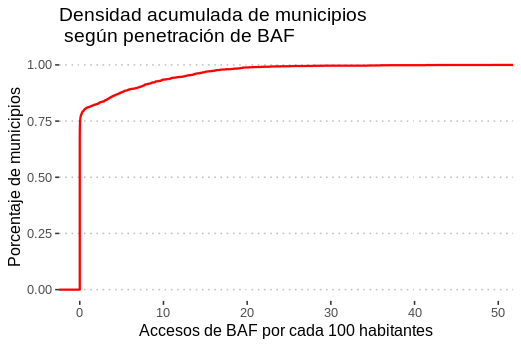
\includegraphics[width=0.9\linewidth]{images/cumulative_dens_pen.png}
	\caption{Distribución acumulada de municipios según su penetración de BAF}
	\label{fig:cumulative}
\end{figure}

Para ilustrar el panorama de la diferencias en la cobertura en los diferentes municipios del país, se construyó la distribución acumulada empírica de los municipios según su penetración de accesos de BAF basados en cable coaxial y fibra óptica. Se aprecia que dicho parámetro oscila entre 0 y cerca de 50 accesos por 100 habitantes a nivel municipal, además casi el 75\% de los municipios del país no cuenta con penetración de BAF. En contraste, únicamente 10\% de los municipios supera los 10 accesos de BAF de este tipo por cada 10 habitantes.

En complemento, también se elaboraron mapas de calor\footnote{Librearía \emph{mxmaps}, disponible a través de https://www.diegovalle.net/mxmaps/. Por otra parte, una versión interactiva de este mapa se encuentra dispoinble para su consulta en el repositorio de Github que acompaña a este documento \url{https://github.com/czammar/BandaAnchaFija/blob/master/Mapas/Penetracion_BAF_xcada100Habitantes_062019.html}} que responde a la cantidad de accesos de BAF (basados en fibra óptica y cable coaxial) por cada 100 hogares eligiéndose tres zonas diferentes del país: i) península de Baja California (figura \ref{fig:pen_habs_penbc}) y iii) Ciudad de México (figura \ref{fig:pen_habs_cdmx}).

 En términos generales, para las zonas de la península se aprecia mayor penetración en municipios fronterizos o zonas turísticas. Para la zona de la Ciudad de México, se aprecia una mayor penetración en la delegaciones Benito Juárez, Cuahutemoc  y Miguel Hidalgo, mientras que Milpa Alta y Tláhuac son las zonas con menores niveles observados.

\subsubsection{Estratificación de municipios de acuerdo a su nivel de cobertura BAF}

Dado que, como se hizo notar en la sección previa, la cobertura de los municipios es heterogénea, para estudiarla se categorizará a cada municipio del país acuerdo a su nivel de penetración de banda ancha fija, con referencia al valor promedio de los países miembros de la OCDE (30.92 accesos por cada 100 habitantes), como se aprecia en la tabla 
\ref{table:clasifpen}.

\begin{table}[tbhp]
	\centering
	\caption{Niveles de penetración en un municipio\label{table:clasifpen}}
	\begin{tabular}{@{}ll@{}}
		\toprule
		%\rowcolor[HTML]{EFEFEF} 
		Nivel de penetración & Rango  de penetración            \\ \midrule
		Muy Alta  & $Penetracion > Media \ OCDE$         \\ 
		%\rowcolor[HTML]{EFEFEF} 
		Alta    & $20 < Penetracion \leq Media \ OCDE$ \\ 
		Media    & $10 < Penetracion \leq 20$  \\ 
		%\rowcolor[HTML]{EFEFEF} 
		Baja      & $0 < Penetracion \leq 10$  \\ 
		%\rowcolor[HTML]{EFEFEF} 
		Nula      & $Penetracion =0$            \\ \bottomrule
	\end{tabular}
	%\addtabletext{Clasificación de municipios según su rango de penetración de BAF}
\end{table}


\subsubsection{Distribución de poblacion y hogares}

Como se ha mencionado previamente la distribución de población y hogares son factores que los operadores de telecomunicaciones toman en cuenta para realizar sus despliegues, y por lo tanto es un factor a considerar para explicar el nivel de penetración de BAF en municipios. Sin embargo, que un porcentaje de la población mayor al 16\% habita 1,698 municipios donde no existen accesos de las tecnologías cable coaxial ni fibra óptica; en contraste los municipios con alta nivel de penetración agrupan únicamente a 2.4\% de la población del país.

\begin{table}[tbhp]
\centering
\caption{Distribución de población y hogares según nivel de penetración de BAF en municipios}
\label{tab:dist_pob_hogs}
\begin{tabular}{@{}lcccc@{}}
	\toprule
	Penetracion & \multicolumn{1}{l}{\# Municipios} & \multicolumn{1}{l}{\% Municipios} & \multicolumn{1}{l}{\% Poblacion} & \multicolumn{1}{l}{\% Hogares} \\ \midrule
	Nula & 1,686 & 68.1 & 16.4 & 15.5 \\
	Baja & 629 & 25.4 & 38.5 & 37.4 \\
	Media & 134 & 5.4 & 35.4 & 36.3 \\
	Alta & 20 & 0.8 & 7.42 & 7.96 \\
	Muy alta & 8 & 0.3 & 2.4 & 2.85 \\ \bottomrule
\end{tabular}
\end{table}


\subsubsection{Ingreso y penetración}
Del análisis (ver figuras \ref{fig:pen_income} y \ref{fig:pen_smm}) se desprende una relación escalonada, en términos generales, entre el ingreso que de los municipios de México\footnote{Se reitera que en la fuente considerada no se cuentan con datos de 11 municipios del país.}, y el nivel de penetración de BAF basado en fibra óptica y cable coaxial, lo cual sugiere que los despliegues de ambas tecnologías se han focalizado en municipios donde hay mayores ingresos por habitante.



\subsubsection{Densidad de habitantes y penetracion}

De acuerdo a la figura \ref{fig:pen_denhabs}, aunque existe variabilidad considerable en la densidad de habitantes por municipio la información refleja un escalonamiento de conforme al nivel de penetración de BAF en los municipios.

\section{Metodología para inferencia de niveles de cobertura de banda ancha fija en municipios}

En linea con la exposición anterior, se busca explorar la posibilidad de que la información del entorno socio-económico, demográfico y tecnológico de los municipios sirva como una vía que permita inferir el nivel de cobertura actual de los servicios de banda ancha fija que los operadores hayan desplegado a la fecha.

Para ello, se propondrán modelos de aprendizaje de máquina que permitan clasificar a los municipios de acuerdo a las siguientes situaciones:

\begin{itemize}
	\item[\textbf{P1:}] Existe o no penetración de BAF basada en accesos de fibra óptica o cable coaxial. \vspace{-0.3cm}
	\item[\textbf{P2:}] Nivel de penetración de BAF basada en accesos de fibra óptica o cable coaxial, de acuerdo a las especificaciones de la tabla \ref{table:clasifpen}.
\end{itemize}

En ambos casos, la metodología a seguir\footnote{Aunque los pasos se presentan de manera lineal, la implementación requirió iteraciones entre ellos a efector de mejorar el funcionamiento global de las predicciones} es la siguiente:

\begin{itemize}
	\item[\textbf{A}.] Definir los modelos a considerar, \vspace{-0.3cm}
	\item[\textbf{B}.] De entre todas la información reunida, establecer cuales son las variables relevantes a considerar,\vspace{-0.3cm}
	\item[\textbf{C}.] Procesamiento de los datos de manera compatible con sus requerimientos de estos,\vspace{-0.3cm}
	\item[\textbf{D}.] Para la ejecución de cada modelo, realizar un pipeline que permita calibrar los posibles hiper-parámetros de los modelos, considerando la evaluación de los mismos con un métrica establecida a través de validación cruzada,\vspace{-0.3cm}
	\item[\textbf{E}.] Considerar el mejor modelo resultado del pipeline anterior de acuerdo a la métrica predefinida, y\vspace{-0.3cm}
	\item[\textbf{F}.] Analizar los resultados interpretando el funcionamiento de los modelos de aprendizaje de máquina.	
\end{itemize}

A continuación se exponen las consideraciones realizadas para llevar a cabo las fases anterior, en el entendido que la ejecución de estas se realizó a través de diferentes programas implementados en Python.

\subsection{Modelos de aprendizaje de máquina a considerar}

Dado que se trata de problemas clasificación , se estimó pertinente considerar un modelo de referencia (\emph{baseline}) a partir de una regresión logística.

Ahora bien, dado en análisis exploratorio realizado se aprecia que la penetración de banda ancha no guarda necesariamente relaciones lineales con las diferentes variables se estimó que los árboles podrían ser de utilidad en el contexto de \textbf{P1} y \textbf{P2}, por lo cual se estimó pertinente usar los modelos que se describen a continuación:

\subsubsection{Modelo de regresión}

Los modelos regresión de regresión se emplean a problemas de clasificación de $K\geq 1$ clases; es decir se consideran conjuntos de puntos y etiquetas de la forma ${\mathcal D} =\{(x^{(i)}, y^{(i)}) \in \mathbb{R}^n \times \{0,1,2, \ldots, K-1\}: i\in [m] \}$ donde se asume la existencia de una relación funcional en términos probabilísticos $\mathbf{y} = \mathbf{W}^T \mathbf{x} + \epsilon$ donde $\mathbf{W}$ es un vector de pesos y $\epsilon$ representa un error residual.

En el caso en que la respuesta sea binaria ($y\in \{0,1\}$) suele aplicarse el modelo de regresión logística el cual asume que $y$ sigue una distribución Bernoulli, $p(\mathbf{y}| \mathbf{W}, \mathbf{x})= Ber(y|\mu(\mathbf{x}))$ donde la media satisface $\mu(\mathbf{x}) = E[y | \mathbf{x}] = p(y=1|x) =sigm(W^Tx)$\footnote{Función sigmoide dada por $sigm(\eta) = \frac{1}{1+ e^{-\eta}}$}. Dicho modelo predice la etiqueta $\hat{y}(x)$de un punto específico $x$ a través de un umbral $p\in (0,1)$; es decir decide que $\hat{y}(x)=1 \leftrightarrow p(y=1|x)>p$.

Por otra parte, el modelo de regresión multinomial resulta de una generalización de lo anterior, para tratar puntos con múltiples etiquetas ($K>1$). En este caso, la probabilidad de que cada punto pertenezca una clase $k$ se modela con la función $softmax$, esto es $P[y=k] = \frac{\exp(\mathbf{W}_k^T x )}{\sum_{i=1}^{K-1}\mathbf{W}_i^T x}$, donde $W_i$ refiere a la $i$-ésima columna del vector de pesos. En ente sentido, esta familia de modelos predice la etiqueta $\hat{y}(x)$de un punto específico $x$ a través asignándolo a la clase que maximice la probabilidad de pertenencia a ésta.

\subsection{Bosques aleatorios}

En el contexto de problemas de clasificación los árboles son modelos de aprendizaje de máquina que buscan realizar predicciones explorando a los individuos a través de cortes en sus características (variables de entrada) con el objeto de ir dividiendo la muestra, de manera que mediante cortes sucesivos se puedan refinar hasta establecer regiones que caractericen a las predicciones de manera acertada, lo cual 1) permite aproximar relaciones no lineales entre sus variables, y 2) otorga variabilidad en el proceso de su construcción.

Los bosques aleatorios son modelos de ensamble, pues permiten incorporar la información de predicciones de muchos árboles; para disminuir la varianza se recurre a un proceso que induce árboles con menor correlación entre sí. Para ello se considera una colección de muestras bootstrap\footnote{Se refiere a una colección de muestras del conjunto de prueba, elegidas con reemplazo y con la misma cardinalidad que este conjunto en estudio} ${\mathcal D}_1^*, {\mathcal D}_2^*, \ldots, {\mathcal D}_B^*$ proveniente de los puntos de entrenamiento y sus etiquetas ${\mathcal D} =\{(x^{(i)}, y^{(i)})\}_{i=1}^n$, prefijando un número $m$ de ss características. Para cada unas de tales muestras bootstrap se construye un árbol bajo el esquema de que: a)
en cada nodo candidato a particionar, se escogen al azar $m$ variables; 2) de entre ellas se elige la mejor variable y punto de corte (e.g. con un criterio de medida de impureza, coeficiente de Gini, entre otros), 3) repetir 1) y 2) hasta obtener un árbol suficientemente grande.

Ello permite consolidar un sistema de votación entre las predicciones de todos los árboles; de modo que la clase a la que pertenece un punto específico se estima como aquella a la que predijeron en mayor medida los árboles construidos en el proceso previamente descrito; es decir mediante la expresión $T^*(x) = argmax_k \{ \# \{b |T_b^*(x)=k; b=1,\ldots, B\}\}.$


\subsection{Gradient tree boosting}
El algoritmo de potenciación de gradiente de árboles (\emph{gradient tree boosting}) es una técnica de aprendizaje de máquina que parte de la premisa de que al combinar de manera aditiva una cantidad de modelos base (árboles) se puede obtener un modelo con mejoras en sus capacidades de aprendizaje (\cite{Chen:2016:XST:2939672.2939785}). Ello equivale a que dado un conjunto de datos,${\mathcal D} =\{(\mathbf{x_i}, y_i) : \mathbf{x_i}\in  \mathbb{R}^m, y_i\in  \mathbb{R} \}$ con $|{\mathcal D}|$, la predicción resulta de un ensamble $\hat{y}_i = \sum_{k=1}^K f_k(x_i), f_k \in \mathcal{F}$, donde $K$ es el número de árboles, $f_k$ se refiere a una familia de modelos base de tipo árbol, $\mathcal{F}=\{ f(\mathbf{x}) = w_{q(\mathbf{x})} :  T\in \mathbb{N}, q: \mathbb{R}^m \rightarrow \{1,2,\cdots,T\} ,  w\in \mathbb{R}^T  \}$, siendo $T$ el número de hojas de un árbol $f_k$ y $q$ una función que representa su estructura\footnote{Estableciendo una regla de asociación entre un punto del espacio y el índice de la hoja del árbol a la que corresponde} y $w$ una colección de pesos sobre sus hojas\footnote{En un ejemplo específico, se emplean reglas de decisión sobre la estructura de los árboles a elegir, para clasificarlos respecto a la elección de sus hojas y crear una predicción sumando los pesos de las mismas}.

Desde una perspectiva teórica, el aprendizaje del modelo se logra a través de la optimización de una función objetivo ${\mathcal L}(\phi)$ que incorpora a una función de pérdida $l(y_i, \hat{y}_i)$ convexa 
y un término $\Omega$ que penaliza la complejidad del modelo y permite su regularización para evitar sobre-ajuste. Sin embargo, dado que puede ser difícil de minimizarla con métodos tradicionales, a través del algoritmo en comento se plantea aproximar dicha función en el proceso de entrenamiento de una manera aditiva, iniciando desde una predicción constante y añadiendo una función en cada paso; es decir para $\hat{y}_i^{(t)}$ la predicción del $i$-ésimo individuo en la $t$-ésima etapa de entrenamiento realizar la minimización de:
\begin{equation}\label{aprox_gboost}
{\mathcal L}^{(t)} = \sum_{i=1}^n l(y_i, \hat{y}_i^{(t-1)}+f_t(\mathbf{x}_i)) + \sum_{k=1}^K \Omega(f_k)
\end{equation}

Pero considerando únicamente los términos de primer y segundo orden de la función de pérdida, $g_i = \partial_{\hat{y}_i^{(t-1)}} l(y_i, \hat{y}_i^{(t-1)})$  $h_i = \partial_{\hat{y}_i^{(t-1)}}^2 l(y_i, \hat{y}_i^{(t-1)})$. Dicha estrategia permite encontrar una expresión simplificada de la aproximación de (\ref{aprox_gboost}):
\begin{equation}
\tilde{{\mathcal L}}^{(t)} =\sum_{i=1}^n [g_i f_t(x_i) + \frac{1}{2} h_i f_t^2(x_i)] + \Omega(f_t) \approx {\mathcal L}^{(t)}
\end{equation}

Lo cual equivale a que si $I_j := \{i|q(x_i)=j\}$, entonces:
\begin{equation}
\tilde{{\mathcal L}}^{(t)} =\sum^T_{j=1} [(\sum_{i\in I_j} g_i) w_j + \frac{1}{2} (\sum_{i\in I_j} h_i + \lambda) w_j^2 ] + \gamma T
\end{equation}

A partir de ella, para una estructura fija de un árbol $q(\mathbf{x})$, se puede obtener una expresión cerrada del peso $w_j^*$ en la $j$-ésima hoja de dicho árbol, donde si $G_j := \sum_{i\in I_j} g_i$ y $H_j = \sum_{i\in I_j} h_i$ entonces:
\begin{equation}
w_j^\ast = -\frac{G_j}{H_j+\lambda}
\end{equation}

Así como el cálculo del correspondiente valor óptimo:
\begin{equation}
{\tilde{{\mathcal L}}^{(t)}}(q) = -\frac{1}{2} \sum_{j=1}^T \frac{G_j^2}{H_j+\lambda} + \gamma T
\end{equation}

A partir de esta forma de medir qué tan bueno es un árbol, se puede plantear un algoritmo
para crecer un árbol de la siguiente forma: 1) comenzar con un árbol de profundidad cero, 2) para cada nodo de hoja del árbol, intentar agregar una división (split), 3) evaluar la reducción de la perdida después de agregar la división para decidir si es aceptable con la ecuación:
$$\mathcal{L}_{split} = \frac{1}{2} \left[\frac{G_L^2}{H_L+\lambda}+\frac{G_R^2}{H_R+\lambda}-\frac{(G_L+G_R)^2}{H_L+H_R+\lambda}\right] - \gamma$$

XGBoost\footnote{https://xgboost.readthedocs.io/en/latest/}  es una de las librerías más populares que implementa el algoritmo recién descrito, encontrándose disponible para Python y R.

\subsection{Variables a considerarse en los modelos}

En el caso del \textbf{P1} para clasificar a los municipios por la presencia o no de servicios de BAF basados en fibra óptica, se estimó pertinente considerar a las siguientes variables por municipio: 1) número de hogares, 2) número de habitantes, 3) superficie (en km), 4) densidad de $hogares/km^2$, 5) densidad de $habitantes/km^2$, 6) porcentaje de habitantes de municipio sin educación primaria, 7) años promedio de escolaridad por habitante, 8) porcentaje de hogares sin acceso a electricidad,  9) porcentaje de hogares sin acceso a energía eléctrica, 10) porcentaje de población que vive en localidades de menos de 5,000 habitantes, 11) porcentaje de la población que gana menos de 2 salarios mínimos, 12) ingreso promedio anual per cápita (poder de paridad de compra, expresado en dólares), 13) porcentaje de hogares con servicios de televisión de paga, 14) porcentaje de hogares con servicios de telefonía celular, y 15) porcentaje de hogares con disponibilidad de teléfono fijo.

Dado que en \textbf{P2} se busca clasificar con respecto al nivel específico de penetración de BAF en los municipios se estimó necesario proveer información adicional sobre el nivel de presencia de Internet y el nivel de competencia entre operadores para el despliegue de accesos basados en las tecnologías multi-citadas; ello a través variables descritas para \textbf{P1} añadiendo 16) el porcentaje de hogares con disponibilidad de Internet, y 17) una variable que indica si hay dos o más operadores de telecomunicaciones que proveen servicios de BAF basados en cable coaxial o fibra óptica. 

\subsection{Procesamiento de los datos}

Para los modelos de regresión las variables numéricas fueron estandarizadas aplicando una función z-score para evitar problemas numéricos asociados a su escala. En el caso de los modelos de árboles aleatorios y gradient tree boosting, las covariables no fueron transformadas en el entendido de que el funcionamiento de dichas herramientas es capaz de realizar la clasificación pretendida sin interferencias de escala. 

Para \textbf{P1} la presencia o no de servicios de BAF basados en cable coaxial o fibra óptica se codificó como una variable binaria, que constituye la categoría a ser predecida. En el caso de \textbf{P2} los niveles de penetración se codificaron con una variable categórica donde $0$ refiere a penetración "nula", $1$ a penetración "baja" y así sucesivamente hasta que $5$ alude a penetración "muy alta".

Cabe destacar que los datos de ingreso promedio anual per cápita no se encontraron disponibles para 4 municipios del país; tales fueron excluidos de la modelación.

Por otra parte, se realizó un partición de los datos de manera aleatoria para consolidar un conjunto de entrenamiento y prueba, guardando una relación, de 75\% y 25\%, de manera respectiva.


\subsection{Ajuste de los modelos y calibración de sus hiper-parámetros}

A manera de establecer una métrica que permita comparar entre los modelos a considerar, se estableció al $f1$-score.

Los modelos de regresión fueron ajustados con los datos descritos en la sección previa, usando el método de optimización \emph{lbfgs} para \textbf{P1} y  para \textbf{P2} se consideró a la función softmax para transforma la salida hacia las clases del problema de clasificación.

Para los modelos de árboles aleatorios se ajustaron los pesos de los árboles de manera inversamente proporcionales a las frecuencias de clase en los datos de los municipios para considerar el desbalance en los niveles de penetración de BAF. Además, tales modelos se calibraron los siguientes hiper-parámetros 1) la cantidad de árboles aleatorios a considerar, 2) la profundidad máxima de los árboles a considerar, 3) el mínimo número de muestras necesarias para dividir a un nodo de un árbol.

Por lo que hace a los modelos de gradient tree boosting, se ajustaron los siguientes hiper-parámetros: i) la tasa de aprendizaje,  ii) la reducción de pérdida mínima requerida para realizar una partición adicional en un nodo hoja del árbol, iii) la profundidad máxima de los árboles a considerar, iv) la profundidad máxima de los árboles, v) la proporción del conjunto de entrenamiento que se empleará para muestra y construir los árboles, vi)la proporción de columnas del conjunto de entrenamiento que se usara para construir los árboles, así como vii) la cantidad de árboles aleatorios a considerar.

Para \textbf{P1} y \text{P2}, para la evaluación de la pertinencia de los hiper-parámetros se empleó validación cruzada de 6 hojas.

El detalle del procedimiento usado se puede consultar en los apéndices que acompañan al presente documento.

\subsection{Análisis de resultados}

En el caso de los modelos de regresión logística, se realizó el ajuste sobre el conjunto de entrenamiento, para posteriormente realizar la predicciones correspondiente sobre el conjunto de prueba. 

Por su parte, los modelos de árboles, se ajustaron con los parámetros que obtuvieron mejores resultados sobre el conjunto de entrenamiento a través de validación cruzada y en función de la métrica descrita en la sección previa.

Realizando el ajuste de los modelos con los valores correspondientes a dichos hiper-parámetros sobre el conjunto de entrenamiento, se procedió a comparar los resultados obtenidos por todos los modelos sobre el conjunto de prueba.

Es así que los resultados de la metodología recién descrita para \textbf{P1} y \textbf{P2} se presentan a continuación:

\subsubsection{P1}

Recordemos que este problema aborda la clasificación de un municipio de acuerdo a si hay presencia de penetración de accesos de banda ancha fija basado en las tecnologías de cable coaxial y fibra óptica. 

\begin{table}[tbhp]
	\centering
	\caption{Promedio ponderado de resultados obtenidos para los distintos modelos - P1 }
	\label{tab:p1_results}
	\begin{tabular}{@{}llllll@{}}
		\toprule
		\# & Modelo & Precisión & Recall & $F1$-score & Soporte \\ \midrule
		1 & Logístico & 0.87 & 0.87 & 0.86 & 612 \\
		2 & Bosque Aleatorio & 0.87 & 0.86 & 0.87* & 612 \\
		3 & Gradient Tree Boosting & 0.87 & 0.86 & 0.86 & 612 \\ \bottomrule
	\end{tabular}
\end{table}

A través de la tabla \ref{tab:p1_results} se aprecia que el modelo de bosques aleatorio fue el que obtuvo mejor $F1$-score, a nivel promedio ponderado, sobre el conjunto de prueba, y que el resto de modelos obtuvo valores similares de desempeño.

Sin embargo, al analizar las matrices de confusión (ver figuras \ref{fig:p1_mc_logistic} , \ref{fig:p1_mc_rd} y \ref{fig:p1_mc_xgboost}) se puede como el modelo logístico
acertó en la predicción de más valores que los basados en árboles, mientras que los otros tuvieron menos falsos positivos que éste. Se destaca que las matrices de los modelos basados en árboles son prácticamente iguales, salvo en que la matríz del modelo de gradient tree boosting tuvo un falso positivo más que la proveniente del modelo de bosque aleatorio.

En complemento, a través de los diagramas de feature importance asociados al modelo de gradient tree  boosting, (ver figuras \ref{fig:p1_xgboost_weight}, \ref{fig:p1_xgboost_gain}, \ref{fig:p1_xgboost_cover} presentes en el apéndice) se puede apreciar que el número de hogares, el porcentaje de población del municipio que vive en localidades de menos de 5,000 hogares, la cantidad de habitantes, el ingreso anual per capita y la densidad de hogares son las variables que más aportaron en la reducción de pérdida a la hora de efectuar splits de los árboles del método, es decir, en términos relativos fueron las que más aportaron a la predicción de la existencia de cobertura de BAF.

\subsubsection{P2}

Mediante la tabla \ref{tab:p2_results} se desprende que el modelo de bosques aleatorio fue el que obtuvo mejor $F1$-score, respecto al promedio ponderado, sobre el conjunto de prueba, y que el resto de modelos obtuvo valores similares de desempeño.

\begin{table}[tbhp]
	\centering
	\caption{Promedio ponderado de resultados obtenidos para los distintos modelos - P2}
	\label{tab:p2_results}
	\begin{tabular}{@{}llcccc@{}}
		\toprule
		\# & Modelo & \multicolumn{1}{l}{Precisión} & \multicolumn{1}{l}{Recall} & \multicolumn{1}{l}{$F1$-score} & \multicolumn{1}{l}{Soporte} \\ \midrule
		1 & Logístico (1 vs all) & 0.90 & 0.88 & 0.89 & 612 \\
		2 & Logístico (all vs all) & 0.90 & 0.88 & 0.89 & 612 \\
		3 & Bosque aleatorio & 0.90 & 0.89 & 0.89* & 612 \\
		4 & Gradient Tree Boosting & 0.89 & 0.88 & 0.88 & 612 \\ \bottomrule
	\end{tabular}
\end{table}

Se aprecia que respecto a los resultados obtenidos en el caso anterior, existe un aumento en la métrica de los valores predecidos; presumiblemente derivado de que dimos más información al modelos respecto a la presencia de servicios de Internet en los municipios y sobre la competencia a nivel local entre operadores.

Al revisar las matrices de confusión de esos modelos (véase las figuras \ref{fig:p2_mc_logistic_1toall}, \ref{fig:p2_mc_logistic_alltoall}, \ref{fig:p2_mc_rd} y \ref{fig:p2_mc_xgboost} en el apéndice) se aprecia, en términos generales: a) em general, el modelo de gradient tree boosting fue el único que se equivocó prediciendo la penetración de un municipio a un nivel inmediato superior o inferior, b) ninguno de los modelos pudo predecir acertadamente el nivel de penetración del municipio con penetración muy alta.

Por otro lado, de acuerdo las figuras de feature importance asociados al modelo de gradient tree  boosting, (ver figuras \ref{fig:p2_xgboost_weight}, \ref{fig:p2_xgboost_gain}, \ref{fig:p2_xgboost_cover} presentes en el apéndice) se desprender que la cantidad de operadores presentes en el municipio que tienen instalados servicios de BAF, el porcentaje de disponibilidad de Internet, que el número de hogares y la población son las variables que más aportaron en la reducción de pérdida a la hora de efectuar splits de los árboles del método, es decir, en términos relativos fueron las que más aportaron a la predicción del nivel de cobertura de BAF a nivel municipio.


\subsection{Conclusiones}

En este documento, exploramos el uso de modelos de aprendizaje de máquina para inferir el nivel de penetración de banda ancha de cierto tipo de tecnologías en los municipios del país, referido como la cantidad de acceso por cada 100 habitantes, a partir de datos socio-económicos provenientes fuentes públicas, basándonos en modelos de aprendizaje de tipo logístico y ensambles de árboles.

Aunque existen limitaciones en la precisión alcanzada por estos modelos, sobretodo al no involucrar detalle de la presencia de infraestructura a nivel geográfico, lo mostrado aquí sugiere que este tipo de modelos puede ser una alternativa para inferir el nivel de cobertura en una zona ante la ausencia de datos de despliegue de operadores, que pueda ser de utilidad a tomadores de decisiones, por ejemplo en la implementación de políticas públicas para aumentar el nivel de penetración de banda ancha, en el entendido de que al entrenarse con datos de México, estos modelos podrían ser aplicables a regiones que posean un nivel de madurez semejante para servicios fijos de telecomunicaciones.


\bibliography{ilcss-sample}

\begin{appendices}
	
	\section{Repositorio Github}
	
	El desarrollo de este trabajo se consolidó a través de un repositorio en Github de acceso público: https://github.com/czammar/BandaAnchaFija; este contiene la totalidad de script desarrollados en Bash, R, Python, los mapas interactivos, las versiones en .tex de los documentos así como los datos empleados.
	
	\section{Figuras de análisis exploratorio}

\begin{figure}[tbhp]
	\centering
	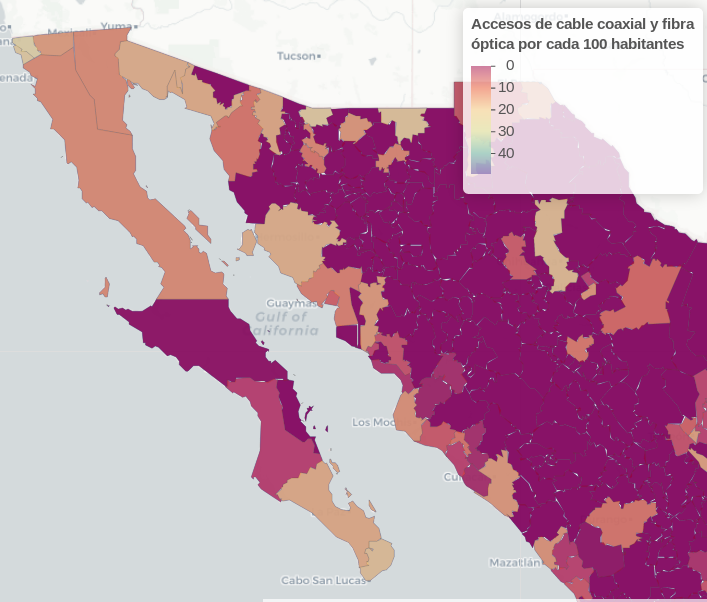
\includegraphics[width=0.9\linewidth]{images/pen_habs_penbc.png}
	\caption{Penetración de cable coaxial y fibra en la península de Baja California}
	\label{fig:pen_habs_penbc}
\end{figure}

\begin{figure}[tbhp]
	\centering
	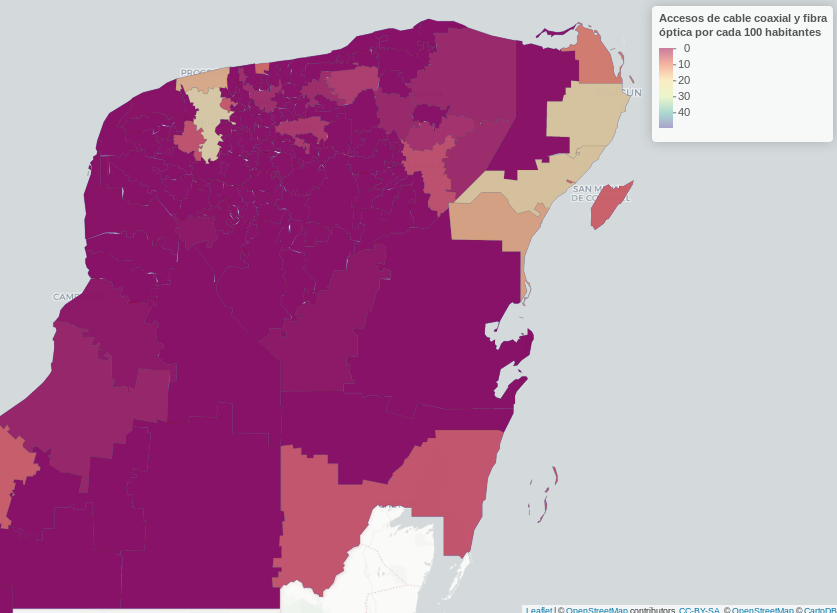
\includegraphics[width=0.9\linewidth]{images/pen_habs_penyuc.png}
	\caption{Penetración de cable coaxial y fibra en la península de Yucatán}
	\label{fig:pen_habs_penyuc}
\end{figure}

\begin{figure}[tbhp]
	\centering
	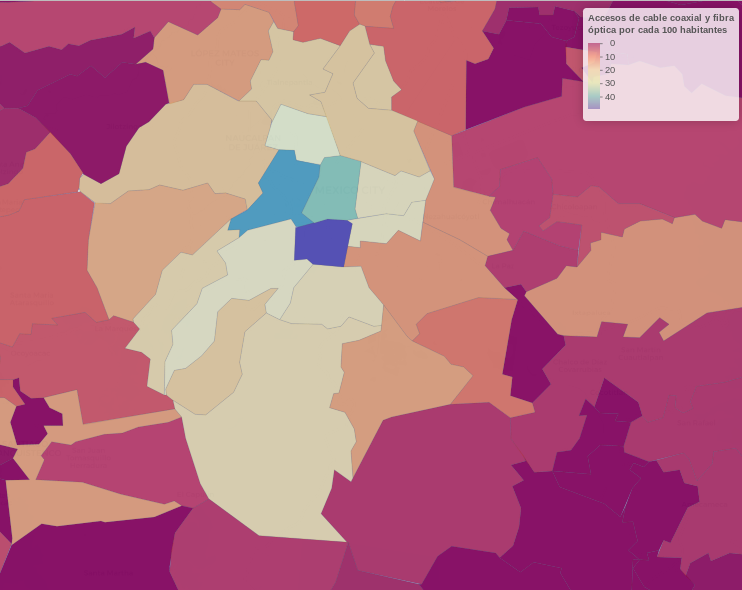
\includegraphics[width=0.9\linewidth]{images/pen_habs_cdmx.png}
	\caption{Penetración de cable coaxial y fibra alrededor de CDMX}
	\label{fig:pen_habs_cdmx}
\end{figure}

\begin{figure}[tbhp]
	\centering
	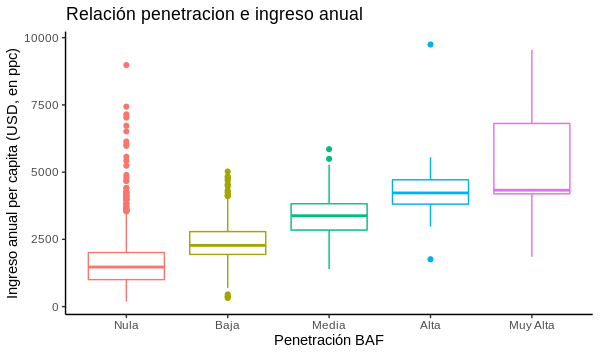
\includegraphics[width=1.0\linewidth]{images/pen_income.png}
	\caption{Penetración BAF Junio 2018 (\cite{IFT2019BIT}) vs Ingreso Anual per capita en municipios (\cite{ONU2015}) }
	\label{fig:pen_income}
\end{figure}

\begin{figure}[tbhp]
	\centering
	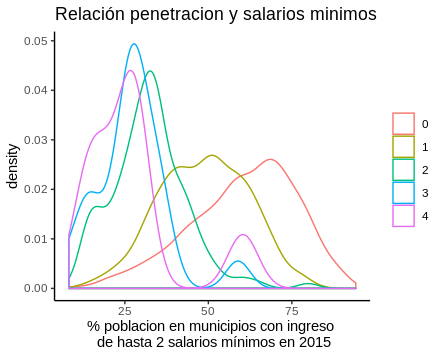
\includegraphics[width=1.0\linewidth]{images/pen_smm.png}
	\caption{Gráfico de densidad del porcentaje de población en municipios que ganaba hasta 2 salarios mínimos(\cite{CONAPO2015}), desagregado por nivel de penetración de BAF. \textbf{Nota:} 0 = Pen. nula, 1= Pen. Baja, ..., 5= Pen. Muy alta}
	\label{fig:pen_smm}
\end{figure}

\begin{figure}[tbhp]
	\centering
	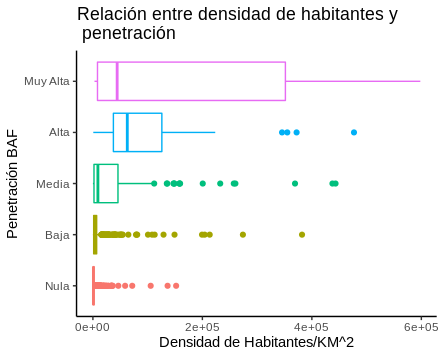
\includegraphics[width=1.0\linewidth]{images/pen_denhabs.png}
	\caption{Densidad de habitantes en municipios vs Penetración BAF Junio 2018 (\cite{IFT2019BIT})}
	\label{fig:pen_denhabs}
\end{figure}
\newpage
\section{Resultados de modelos para P1}

\begin{figure}[tbhp]
	\centering
	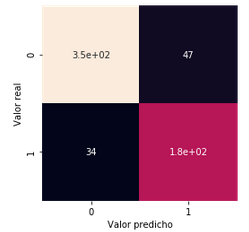
\includegraphics[width=0.6\linewidth]{images/p1_mc_logistic.png}
	\caption{Matriz de confusión del modelo logístico- P1 }
	\label{fig:p1_mc_logistic}
\end{figure}

\begin{figure}[tbhp]
	\centering
	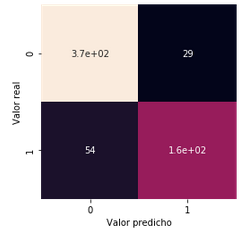
\includegraphics[width=0.6\linewidth]{images/p1_mc_rd.png}
	\caption{Matriz de confusión del modelo de bosque aleatorio- P1 }
	\label{fig:p1_mc_rd}
\end{figure}

\begin{figure}[tbhp]
	\centering
	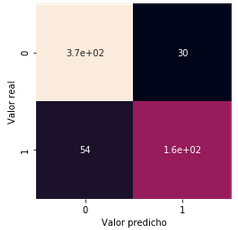
\includegraphics[width=0.6\linewidth]{images/p1_mc_xgboost.png}
	\caption{Matriz de confusión del modelo gradient tree boost- P1 }
	\label{fig:p1_mc_xgboost}
\end{figure}

\begin{figure}[tbhp]
	\centering
	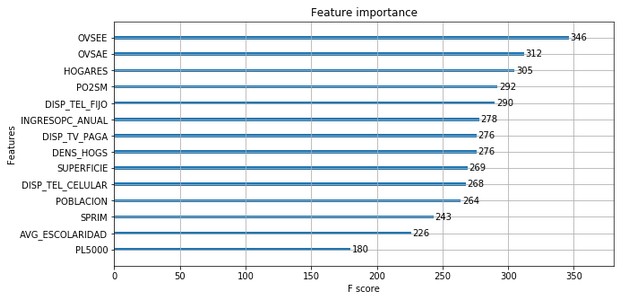
\includegraphics[width=1\linewidth]{images/p1_xgboost_weight.png}
	\caption{Feature importace por "weight" del modelo gradiente tree boosting P1}
	\label{fig:p1_xgboost_weight}
\end{figure}

\begin{figure}[tbhp]
	\centering
	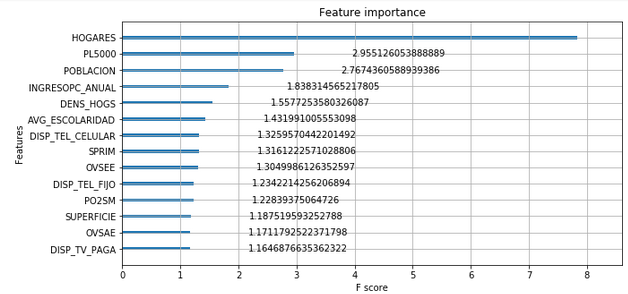
\includegraphics[width=1\linewidth]{images/p1_xgboost_gain.png}
	\caption{Feature importace por "gain" del modelo gradiente tree boosting P1}
	\label{fig:p1_xgboost_gain}
\end{figure}

\begin{figure}[tbhp]
	\centering
	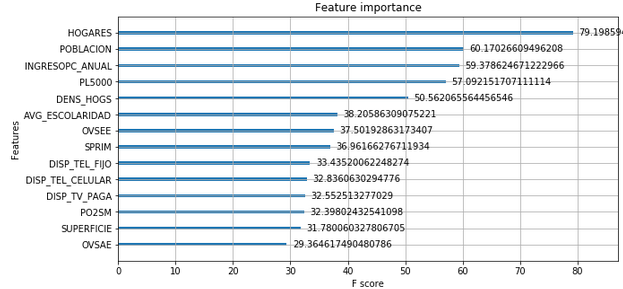
\includegraphics[width=1\linewidth]{images/p1_xgboost_cover.png}\newpage
	\caption{Feature importace por "cover" del modelo gradiente tree boosting P1}
		\label{fig:p1_xgboost_cover}
\end{figure}
	
\section{Resultados de modelos para P2}

\begin{figure}[tbhp]
	\centering
	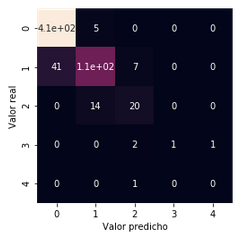
\includegraphics[width=0.6\linewidth]{images/p2_mc_logistic_1toall.png}
	\caption{Matriz de confusión del modelo logístico 1 vs all - P2 }
	\label{fig:p2_mc_logistic_1toall}
\end{figure}

\begin{figure}[tbhp]
	\centering
	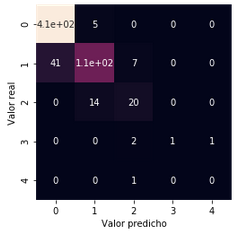
\includegraphics[width=0.6\linewidth]{images/p2_mc_logistic_alltoall.png}
	\caption{Matriz de confusión del modelo logístico all vs all - P2 }
	\label{fig:p2_mc_logistic_alltoall}
\end{figure}

\begin{figure}[tbhp]
	\centering
	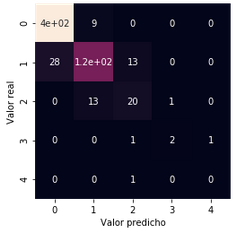
\includegraphics[width=0.6\linewidth]{images/p2_mc_rd.png}
	\caption{Matriz de confusión del modelo de bosque aleatorio - P2 }
	\label{fig:p2_mc_rd}
\end{figure}

\begin{figure}[tbhp]
	\centering
	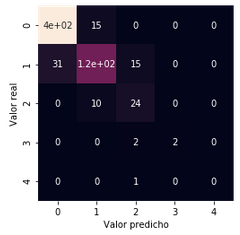
\includegraphics[width=0.6\linewidth]{images/p2_mc_xgboost.png}
	\caption{Matriz de confusión del modelo gradient tree boosting - P2 }
	\label{fig:p2_mc_xgboost}
\end{figure}

\begin{figure}[tbhp]
	\centering
	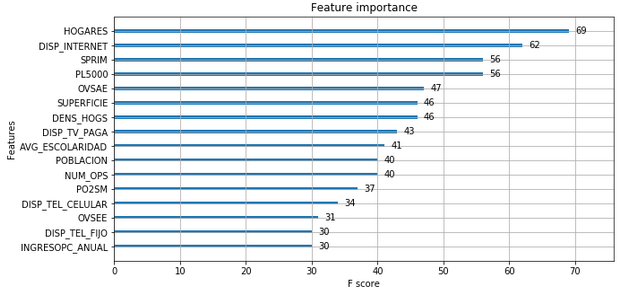
\includegraphics[width=1\linewidth]{images/p2_xgboost_weight.png}
	\caption{Feature importace por "weight" del modelo gradiente tree boosting P2}
	\label{fig:p2_xgboost_weight}
\end{figure}

\begin{figure}[tbhp]
	\centering
	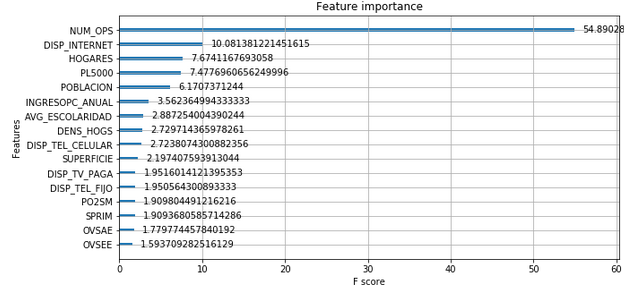
\includegraphics[width=1\linewidth]{images/p2_xgboost_gain.png}
	\caption{Feature importace por "gain" del modelo gradiente tree boosting P2}
	\label{fig:p3_xgboost_gain}
\end{figure}

\begin{figure}[tbhp]
	\centering
	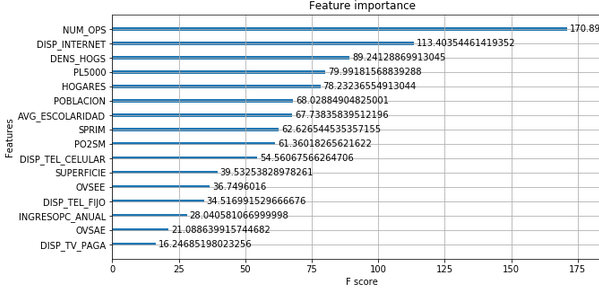
\includegraphics[width=1\linewidth]{images/p2_xgboost_cover.png}\newpage
	\caption{Feature importace por "cover" del modelo gradient tree boosting P2}
\label{fig:p2_xgboost_cover}
\end{figure}

\end{appendices}

\end{document}